\subsection{LI Characteristics}
\label{sec:test:li}

6.25\%

Plot the output light power as a function of forward bias for one of your LEDs (or the standard). Describe the salient features of the graph. [150 words max + Figures].

\begin{figure}[!htb]
\begin{center}
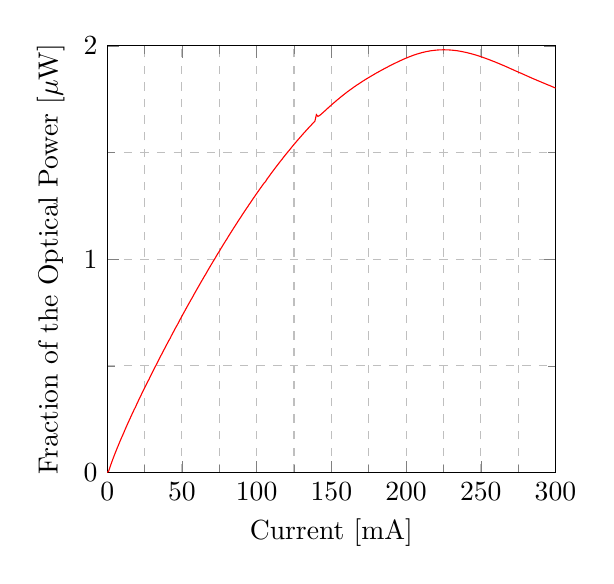
\begin{tikzpicture}

\begin{axis}[
    %title={Temperature dependence of CuSO$_4\cdot$5H$_2$O solubility},
    xlabel={Current [mA]},
    ylabel={Fraction of the Optical Power [$\mu$W]},
    height=7cm,
    width=0.6\textwidth,
    xmin=0, xmax=300,
    ymin=0, ymax=2,
    xtick={0, 50, 100, 150, 200, 250, 300},
    ytick={0, 1, 2},
    legend pos=south east,
    ymajorgrids=true,
    yminorgrids=true,
    xmajorgrids=true,
    xminorgrids=true,
    minor tick num=1,
    grid style=dashed,
]

\addplot[color=red]
  coordinates {
  (-5,-0.0014759999999999999)
  (-4,-0.000519)
  (-3,-0.0004969999999999999)
  (-2,-0.00052)
  (-1,-0.0006670000000000001)
  (0,0.000783)
  (1,0.00598)
  (2,0.027376)
  (3,0.04754)
  (4,0.066299)
  (5,0.084577)
  (6,0.102171)
  (7,0.11938700000000001)
  (8,0.136461)
  (9,0.153228)
  (10,0.169046)
  (11,0.184622)
  (12,0.20156500000000002)
  (13,0.217405)
  (14,0.233166)
  (15,0.24842799999999998)
  (16,0.26369400000000004)
  (17,0.278968)
  (18,0.29378899999999997)
  (19,0.307402)
  (20,0.323493)
  (21,0.338117)
  (22,0.352659)
  (23,0.36718999999999996)
  (24,0.381472)
  (25,0.395729)
  (26,0.409904)
  (27,0.42409)
  (28,0.436924)
  (29,0.452104)
  (30,0.466092)
  (31,0.479788)
  (32,0.49353600000000003)
  (33,0.506934)
  (34,0.520937)
  (35,0.534549)
  (36,0.548228)
  (37,0.561623)
  (38,0.5751210000000001)
  (39,0.5885130000000001)
  (40,0.601862)
  (41,0.615141)
  (42,0.627264)
  (43,0.641607)
  (44,0.6545989999999999)
  (45,0.6677379999999999)
  (46,0.680899)
  (47,0.692817)
  (48,0.706773)
  (49,0.719723)
  (50,0.732565)
  (51,0.745255)
  (52,0.758158)
  (53,0.7707909999999999)
  (54,0.783367)
  (55,0.795961)
  (56,0.8085800000000001)
  (57,0.820235)
  (58,0.8334119999999999)
  (59,0.845796)
  (60,0.858146)
  (61,0.870276)
  (62,0.882655)
  (63,0.894822)
  (64,0.906878)
  (65,0.919052)
  (66,0.930323)
  (67,0.943036)
  (68,0.954967)
  (69,0.9669690000000001)
  (70,0.978702)
  (71,0.990449)
  (72,1.0013960000000002)
  (73,1.013844)
  (74,1.025509)
  (75,1.03608)
  (76,1.048504)
  (77,1.059928)
  (78,1.0714)
  (79,1.0826360000000002)
  (80,1.093375)
  (81,1.105218)
  (82,1.116314)
  (83,1.127405)
  (84,1.138521)
  (85,1.149475)
  (86,1.1602780000000001)
  (87,1.171338)
  (88,1.182134)
  (89,1.192872)
  (90,1.203456)
  (91,1.214204)
  (92,1.2248050000000001)
  (93,1.235303)
  (94,1.245426)
  (95,1.256145)
  (96,1.266407)
  (97,1.276838)
  (98,1.2870100000000002)
  (99,1.297112)
  (100,1.3073)
  (101,1.31731)
  (102,1.327255)
  (103,1.3371870000000001)
  (104,1.346989)
  (105,1.356678)
  (106,1.364087)
  (107,1.375857)
  (108,1.384767)
  (109,1.3948280000000002)
  (110,1.4043700000000001)
  (111,1.413621)
  (112,1.422941)
  (113,1.4323000000000001)
  (114,1.4414440000000002)
  (115,1.450528)
  (116,1.4595879999999999)
  (117,1.4680039999999999)
  (118,1.477431)
  (119,1.486253)
  (120,1.494891)
  (121,1.503474)
  (122,1.51153)
  (123,1.520628)
  (124,1.529079)
  (125,1.537574)
  (126,1.5458049999999999)
  (127,1.554078)
  (128,1.562252)
  (129,1.570135)
  (130,1.578135)
  (131,1.58621)
  (132,1.593987)
  (133,1.601695)
  (134,1.609449)
  (135,1.6170930000000001)
  (136,1.6240409999999998)
  (137,1.632066)
  (138,1.639457)
  (139,1.646734)
  (140,1.6774170000000002)
  (141,1.6691939999999998)
  (142,1.67268)
  (143,1.6783130000000002)
  (144,1.684519)
  (145,1.690801)
  (146,1.696871)
  (147,1.703634)
  (148,1.709874)
  (149,1.716151)
  (150,1.722398)
  (151,1.72858)
  (152,1.73454)
  (153,1.740612)
  (154,1.7465810000000002)
  (155,1.752078)
  (156,1.758152)
  (157,1.7637779999999998)
  (158,1.76935)
  (159,1.77481)
  (160,1.780345)
  (161,1.785686)
  (162,1.790685)
  (163,1.795912)
  (164,1.800586)
  (165,1.805884)
  (166,1.810724)
  (167,1.81558)
  (168,1.82014)
  (169,1.8247879999999999)
  (170,1.829486)
  (171,1.833919)
  (172,1.838367)
  (173,1.8428360000000001)
  (174,1.847)
  (175,1.851177)
  (176,1.8554599999999999)
  (177,1.8594950000000001)
  (178,1.863529)
  (179,1.867809)
  (180,1.871826)
  (181,1.875663)
  (182,1.879619)
  (183,1.8834730000000002)
  (184,1.887251)
  (185,1.8911010000000001)
  (186,1.894866)
  (187,1.898223)
  (188,1.902201)
  (189,1.905752)
  (190,1.909238)
  (191,1.912906)
  (192,1.9163109999999999)
  (193,1.919673)
  (194,1.923133)
  (195,1.926519)
  (196,1.929702)
  (197,1.932993)
  (198,1.936236)
  (199,1.939221)
  (200,1.9421950000000001)
  (201,1.944989)
  (202,1.948101)
  (203,1.950615)
  (204,1.9534349999999998)
  (205,1.955965)
  (206,1.958264)
  (207,1.9606929999999998)
  (208,1.9627859999999997)
  (209,1.964809)
  (210,1.9668530000000002)
  (211,1.9687070000000002)
  (212,1.970365)
  (213,1.9720060000000001)
  (214,1.973468)
  (215,1.9747480000000002)
  (216,1.976153)
  (217,1.977108)
  (218,1.9779870000000002)
  (219,1.978827)
  (220,1.9795939999999999)
  (221,1.9802180000000003)
  (222,1.980754)
  (223,1.9810219999999998)
  (224,1.981178)
  (225,1.981398)
  (226,1.9812699999999999)
  (227,1.980983)
  (228,1.980873)
  (229,1.9805640000000002)
  (230,1.9799190000000002)
  (231,1.979411)
  (232,1.978652)
  (233,1.977833)
  (234,1.9770360000000002)
  (235,1.9759920000000002)
  (236,1.974693)
  (237,1.9734980000000002)
  (238,1.972148)
  (239,1.9705450000000002)
  (240,1.969024)
  (241,1.967492)
  (242,1.965611)
  (243,1.9639649999999997)
  (244,1.962118)
  (245,1.9600659999999999)
  (246,1.9580579999999999)
  (247,1.95609)
  (248,1.9538149999999999)
  (249,1.9515209999999998)
  (250,1.9492820000000002)
  (251,1.946974)
  (252,1.944379)
  (253,1.941871)
  (254,1.939252)
  (255,1.936618)
  (256,1.9339979999999999)
  (257,1.9312509999999998)
  (258,1.928425)
  (259,1.9257980000000001)
  (260,1.922955)
  (261,1.919951)
  (262,1.9172410000000002)
  (263,1.914196)
  (264,1.911133)
  (265,1.908372)
  (266,1.905305)
  (267,1.9022)
  (268,1.899225)
  (269,1.896101)
  (270,1.8926509999999999)
  (271,1.889729)
  (272,1.886485)
  (273,1.883262)
  (274,1.880274)
  (275,1.877184)
  (276,1.874037)
  (277,1.871232)
  (278,1.8680420000000002)
  (279,1.864937)
  (280,1.8617320000000002)
  (281,1.858662)
  (282,1.855412)
  (283,1.852364)
  (284,1.849227)
  (285,1.846035)
  (286,1.843167)
  (287,1.840312)
  (288,1.837189)
  (289,1.834391)
  (290,1.8313769999999998)
  (291,1.828379)
  (292,1.8254549999999998)
  (293,1.822578)
  (294,1.81952)
  (295,1.8165740000000001)
  (296,1.8140090000000002)
  (297,1.810908)
  (298,1.807922)
  (299,1.804923)
  (300,1.80201)
};
  % \addlegendentry{$16\mu m$}


\end{axis}
\end{tikzpicture}

\caption{Fraction of the optical power plotted against the forward current of the LED showing the optical power peak at $220mA$}
\label{fig:li}
\end{center}
\end{figure}


The optical power was measured against current from $0mA$ to $300mA$. As described in section \ref{sec:test:apparatus}, the power measured is not the total output power but a fraction. The results measurements are plotted in \ref{fig:li}. This figure shows the optical power increase from $0mA$ to $220mA$ before decreasing again as the current increases to $300mA$. The peak power is not of any particular interest since it is not absolute but the current at which it occurs, $200mA$, is.
